\documentclass{jsarticle}
\usepackage{../stylesheet/semi}
\graphicspath{{../image/}}

\begin{document}

\日付{2018/07/17}
\氏名{阿部 希駿}
\タイトル{卒業研究進捗報告}

\semi

\section{テーマ}
学習前に全体像を理解することの内容理解への有用性

\section{背景・目的}
国際数学・理科教育動向調査(TIMSS2015)が中学生を対象に実施したアンケートによると,数学や理科を勉強すると日常生活に役立つと考えている学生の割合が国際平均に対し大幅に下回っていることがわかる. \cite{timss} このことからその学習を行う目的を含む学習内容の繋がりや全体像が不透明なまま学習している学生が多いと考えられる.

そこで本研究では各要素の学習を行う前に各要素ごとの繋がりなどの全体像を説明することによって,理解の促進に繋がると仮定し,実験を行う.



\begin{figure}[H]
\begin{minipage}{0.5\hsize}
\begin{center}
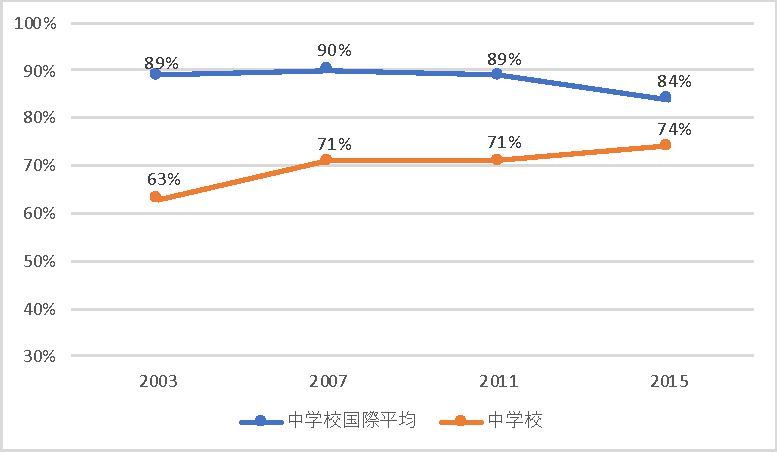
\includegraphics[width=8cm]{0717-1.pdf}
\end{center}
\caption{数学を勉強すると日常生活に役立つか}
\end{minipage}
\begin{minipage}{0.5\hsize}
\begin{center}
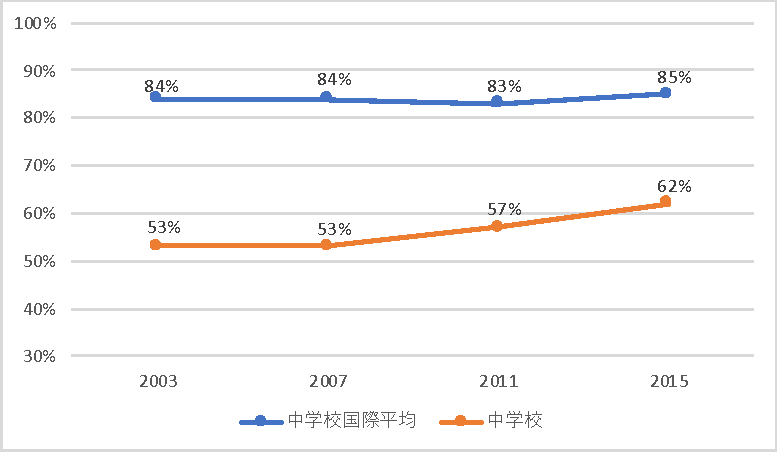
\includegraphics[width=8cm]{0717-2.pdf}
\end{center}
\caption{理科を勉強すると日常生活に役立つか}
\end{minipage}
\end{figure}

\section{実験方法}
2018年度後期の情報数学応用の講義履修者を対象に情報数学応用の9週目と10週目の講義にて実験を行う.

\subsection{具体的な流れ}
ここでは金曜1限の履修者と金曜2限の履修者をそれぞれA群,B群と表記する.


9週目の「ハッシュ値と暗号」の講義の最初にA群のみ10週目の「公開鍵暗号の応用
」を含めた全体的な流れについて受講者に対して説明を行う.10週目の講義の終わりにA群,B群共に小テストを行い,結果を比較する.


\section{今後の課題}

\begin{enumerate}
\renewcommand {\labelenumi}{(\arabic{enumi})}
\item 授業前に説明する内容を考える.
\item 小テストを作成する.
\item 評価方法を考える.
\end{enumerate}




\begin{thebibliography}{99}
\bibitem{timss}
 “国際数学・理科教育動向調査(TIMSS2015)のポイント”. 文部科学省.  \url{http://www.mext.go.jp/component/a_menu/education/micro_detail/__icsFiles/afieldfile/2016/12/27/1379931_1_1.pdf},(参照 2018-7-16)

\end{thebibliography}

\end{document}